
This chapter describes the annotation of events, argument fillers and event co-reference (in the form of Event Hoppers).

\section{What is an event?}

\subsubsection{Conceptually: events in economic news}

An event is a textual description of a real-world occurrence that involves multiple participants.
An event describes what has happened, who was involved, at what time, in which place.
Deals, employee changes, product launches, elections, company mergers or lawsuits are the some intuitive examples of what constitutes an event in economic news. 

\subsubsection{Technically: features of an event}

Technically, an event is always described explicitly in the text:
First, the presence of an event is indicated by a lexical \textbf{trigger.}
Second, each event belongs to a certain \textbf{type and subtype}.
Events outside the typology are not tagged.
We count 12 types and 42 subtypes (see appendix \ref{app/mEREcator_type_table}). 
Third, we want to find the entities (people, companies, organizations, etc.) that participate in the event (so-called \textbf{arguments}).
Fourth, we give the event a \textbf{realis} value that indicates if the event has actually happened or not.
We also perform event co-reference to link event mentions to each other if they refer to the same event.

In the following sections, we explain these elements in detail.

\section{Event triggers}

The trigger of an event is the \textbf{minimal span of text} (a single word or a small phrase) that most succinctly expresses the occurrence of an event.
It is often the main verb describing an action or a state.
Generally, we think of the trigger as the word that most strongly refers to an event.
In the examples below (and throughout this document), event triggers are \anntrg{underlined.}
We also indicate the \type{type and subtype} of most events in the example sentences.

\begin{exe}
    \ex\label{ex/verb1} \annxpl{On Monday, shares of biopharmaceutical company Celgene \anntrg{tumbled}}
        \expl the \textbf{verb} \anntrg{tumbled} is the trigger of a \type{Conflict.Attack} event.
    \ex\label{ex/noun1} Noun: \annxpl{[..] AA's exclusive airline \anntrg{sponsorship deal} with the World Series champion Cubs.}
        \expl the noun \anntrg{sponsorship deal} is the trigger of a \type{CSR/Brand} event.
    \ex\label{ex/noun2} \annxpl{Viscen is revealed to be the \anntrg{buyer} of the ACX directories.}
        \expl the \textbf{noun} \anntrg{buyer} is the trigger of a \type {MA.Acquisition} event.
\end{exe}

\subsection{What forms do event triggers take?}

As examples \ref{ex/verb1} and \ref{ex/noun1} show, the trigger can be a \textbf{verb}, but also a \textbf{noun}, \textbf{pronoun} or a past or present \textbf{participle} or \textbf{adjective} in modifier position.

\begin{exe}
    \ex\label{ex/verb2} Verb: \annxpl{The FDA did not \anntrg{approve} JNJ's new medicine.}
    \ex\label{ex/noun2} Noun: \annxpl{The \anntrg{acquisition} of ACX went over without a problem.}
    \ex\label{ex/adjective} Adjective: \annxpl{The \anntrg{banktrupt} firm left investors angry.}
\end{exe}

We typically think of events as processes or actions; but we also tag states that result from taggable events.
As shown by the examples below, resultative events can be predicate adjectives, participles used as modifiers or even present participles that denote an action currently in progress.

\begin{exe}
    \ex\label{ex/predicateadjective} Predicate adjective: \annxpl{The firm is \anntrg{bankrupt.}}
    \ex\label{ex/npadjective} Nominal modifier adjective: \annxpl{The \anntrg{bankrupt} firm leaves many angry investors behind.}
    \ex\label{ex/presentparticiple} Present participle: \annxpl{The firms are currently \anntrg{merging}.}
\end{exe}

As resultative states these examples can be paraphrased as "the state of having gone bankrupt" or "the state of having been merged".
Always tag both on-going events and resultative events.

Anaphors of events such as \textbf{pronouns and definite descriptions} of previously mentioned events are also tagged.

\begin{exe}
    \ex\label{ex/pronoun1} Pronoun: \annxpl{The firm went \anntrg{bankrupt.} \anntrg{It} was a great loss for many of the early-stage investors.}
        \expl pronoun \anntrg{It} refers to a previous \type{Bankruptcy} event and is tagged.
    \ex\label{ex/pronoun1} Definite noun phrase: \annxpl{Amazon \anntrg{launched} its own smartphone. \anntrg{It} was a festive \anntrg{affair}.}
        \expl pronoun \anntrg{It} and definite noun \anntrg{affair} refers to a previous event \type{Product.Launch}.
\end{exe}

Anaphoric triggers, i.e. \anntrg{it} and \anntrg{affair} do not require argument fillers.
They are the same type and subtype as the event they refer.

% Comes from official rERE gl's p 11.

\subsection{Finding the right trigger}

Identifying the trigger of events is often straightforward, as in example \ref{ex/mainverb} above. Just as often, we find a number of words that could be marked as a trigger, or an event is described in such a way that picking a single word as a trigger does not feel right. As a rule of thumb, we keep triggers as small as possible; in this section, we describe procedures to find the right trigger when it is not obvious.

Practically, annotators read the full article text using the event typology as a guiding reference.
During first reading(s) they note possible events mentioned in the article.
We advice annotators to focus on identifying types first and only assign subtypes after triggers have been found.

Next they attentively go over the article a second time and looking for the lexical triggers.
Noting the triggers, annotators double check their spans.

% \subsubsection{Triggers as contiguous groups of words}

% Is the trigger an uninterrupted group of words?

% An event can be described by a group of words such that it is impossible to pick one word without losing the meaning of the phrase.
% In that case, the trigger is the entire phrase.
% Like many aspects of annotation, this is often subjective; we encourage annotators to use their best judgment based on the examples in this document -- keeping in mind that triggers should not be longer than they absolutely need to be.

% \begin{exe}
%     \ex \annxpl{Hoe zijn de Spaanse autoriteiten de Catalaanse ex-minister-president Carles Puigdemont \anntrg{op het spoor gekomen?}}
%         \expl \type{Justice.Investigation}
%     \ex \annxpl{De soldaten \anntrg{zijn weer thuis.}}
%         \expl None of the words in this group by itself carry the meaning of movement.
%         \expl \type{Movement.TransportPerson}
% \end{exe}

\subsubsection{Picking a word from multiple possible trigger words}

There may still be situations where you can reasonably identify multiple different words for a single event trigger. We provide a few rules in these cases to avoid confusion. As a general rule-of-thumb: Always select the smallest meaningful lexical unit as an event trigger.
\\\\
\noindent\textbf{The Stand-Alone Noun Rule}:
In \textbf{verb+noun} constructions, we will simply select the noun whenever that noun can be used by itself to refer to the event.
If the verb+noun cannot be reduced without loosing the event meaning multiple words will be tagged.

\begin{exe}
    \ex \annxpl{Foo Corp. had previously \textit{filed} \anntrg{Chapter 11} in 2001.}
        \expl the \textbf{noun} \anntrg{Chapter 11} not verb+noun \textit{filed Chapter 11} is the trigger as per the Stand-Alone Noun Rule.
    \ex \annxpl{The company had to \textit{pay a} \anntrg{fine} of 300.000EUR.}
        \expl the \textbf{fine} \anntrg{Chapter 11} not verb+noun \textit{pay a fine} is the trigger as per the Stand-Alone Noun Rule.
\end{exe}

\noindent\textbf{Stand-Alone Adjective Rule}:
In \textbf{verb+X+noun} constructions, when a verb and an adjective are used together to express the occurrence of an event, the adjective will be chosen as the trigger whenever it can stand alone to express the resulting state brought about by the event.

\begin{exe}
    \ex \annxpl{The negative findings left 3 projects \anntrg{disapproved}.}
        \expl the \textbf{adjective} \anntrg{disapproved} not verb+X+adjective \textit{left 3 projects} is the trigger as per the Stand-Alone Adjective Rule.
\end{exe}

\noindent\textbf{Main Verb Rule}: When several verbs are used to together to express an event, only the main verb is the trigger.
\begin{exe}
    \ex \annxpl{XYZ Corp. \textit{announced} \annxpl{laying off} 37 workers in the Chicago facility.}
    \ex \annxpl{John D. Idol will \anntrg{take over} as Chief Executive.}
    \ex \annxpl{XYZ Corp \anntrg{laid} Jane off.}
    \ex \annxpl{John D. Idol had \anntrg{taken} the company over.}
\end{exe}

\noindent\textbf{Contiguous Verb+Particle/Verb+Adverb Rule}: In \textbf{verb+particle and verb+adverb} constructions we will tag main verb and particle together only if the words occur contiguously. If they are interrupted we only annotate the verb.
\begin{exe}
    \ex \annxpl{Jane was \anntrg{laid off} by XYZ Corp.}
    \ex \annxpl{John D. Idol will \anntrg{take over} as Chief Executive.}
    \ex \annxpl{XYZ Corp \anntrg{laid} Jane off.}
    \ex \annxpl{John D. Idol had \anntrg{taken} the company over.}
\end{exe}

\subsection{Multiple events within a sentence}
Do not confuse cases where there multiple possible triggers for the same event within the same sentence with cases where there multiple events expressed in the same sentence.
Multiple events can be expressed in the same sentence.

This usually both in complex sentences, i.e. with coordinated (\textit{and, or, but, for, etc.}) and subordinated (if, that, because, where, etc.) clauses.
But also in simplex sentences consisting of one clause.

\begin{exe}
    \ex \annxpl{The \anntrg{product launch} caused a rise in \anntrg{revenue} and \anntrg{sales}.}
    \ex \annxpl{John D. Idol will \anntrg{take over} as Chief Executive.}
\end{exe}

Sometimes multiple events are triggered by adjectives sharing the same verb. Tag each adjective as a seperate event.

\section{Realis}

The Realis attribute indicates how `real' the event is. \textbf{Actual} events are attested to have occurred in real life; the author asserts with certainty that they have happened. Most events you will find are Actual. \textbf{Generic} events also actually happen, but they do not refer to single specific events. They describe things that happen without referring to a specific instance. For instance, in example \ref{ex/generic_realis}, the act of smuggling is habitual and not specific. Finally, a trigger might describe an event that will happen in the future, or might happen at some point, or might have happened in the past, or someone suggests something might happen or has happened. These type of events, along with negated events, go into the realis category \textbf{Other}.

Events that are reported according to some source (as in example \ref{ex/volgens_politie}) also carry a realis attribute of \textbf{Other}.
% I checked the ACE guidelines for this but they have no info at all.

\begin{exe}
    \ex \annxpl{Provincie Oost-Vlaanderen geeft \anntrg{miljoenencadeau} aan projectontwikkelaar. }
        \expl \type{Trans\-action.\-Trans\-fer\-Money, Realis = Actual.}
    
    \ex\label{ex/generic_realis} \annxpl{Drugs worden vaak de grens \anntrg{overgesmokkeld}.}
        \expl \type{Movement.TransportArtifact, Realis = Generic.}

    \ex\label{ex/volgens_politie} \annxpl{Volgens politiebronnen \anntrg{schept} de dader op in de kliniek.}
        \expl \type{Contact.Broad\-cast, Realis = Other.} \annxpl{Volgens politiebronnen} indicates that the event is a claim by police sources. A claim is not sufficient to tag this event as Actual.
    
    \ex \annxpl{President Trump \anntrg{dreigt} ermee Saipov naar Guantanamo te \anntrg{sturen}. }
        \expl \annxpl{Dreigt:} \type{Contact.Broadcast, Realis = Actual.} 
        \expl \annxpl{Sturen:} \type{Movement.\-Trans\-port\-Personnel, Realis = Other.} The first event indicates the second is only something that might happen in the future.
    
    \ex \annxpl{Uiteindelijk werd het geld helemaal niet \anntrg{overgebracht}. }
        \expl \type{Transaction.Trans\-fer\-Money, Realis = Other.} Negated events go into Other.
\end{exe}


\section{Event arguments}

Each event has a number of corresponding arguments. An argument is a participant in the event, like the person or company doing the action, some other piece of information, like the place where the event happens.
We label arguments for each event mention.
For each event, \textbf{arguments fill a number of roles specific to the event type.}
The \type{Conflict.Attack} event type, for instance, asks for an Attacker, a Target, an Instrument, a Place and a Time. 

\textbf{Argument slots can be left empty} if the relevant argument is not mentioned in the sentence. It is possible that some events have no explicit arguments in the sentence: their entire argument list is empty. 

\textbf{Multiple arguments can take the same role.} In example \ref{ex/one_role_two_args}, the \type{Contact.Meet} type asks for an Entity argument, which is a person or organization that attends the meeting. Two are mentioned in this example, so the event carries two Entity arguments. In the same way, there can be more than two Victim arguments to an \type{Attack} event, or more than two defendants in a \type{Justice.Sentence} event.

The list of mEREcator argument roles is given in appendix \ref{app/arg_roles}.

\begin{exe}
    \ex \annxpl{Bij de \anntrg{terreuraanslag} in \emph{New York} zijn \emph{acht mensen} om het leven gekomen.}
        \expl \type{Conflict.Attack, Realis = Actual}
        \expl Attacker = (empty)
        \expl Target = acht mensen
        \expl Instrument = (empty)
        \expl Place = New York
        \expl Time = (empty)
        
    \ex\label{ex/one_role_two_args} \annxpl{\emph{Mark Zuckerberg} heeft een \anntrg{hoorzitting} voor \emph{twee senaatscommissies} in \emph{Washington} \emph{donderdagochtend} al bij al goed doorstaan.}
        \expl \type{Contact.Meet, Realis = Actual}
        \expl Entity = Mark Zuckerberg
        \expl Entity = twee senaatscommissies
        \expl Place = Washington
        \expl Time = donderdagochtend
\end{exe}

In complex sentences, a single argument to an event can be mentioned more than once. In that case, we annotate the mention that is \textbf{closest to the trigger}. We do not annotate the other mention as an argument. The task of linking those two mentions together is left to the entity coreference step.

\begin{exe}
    \ex\label{ex/kim_jong_un} \annxpl{Krijgt president Donald Trump straks een Nobelprijs voor de Vrede als \emph{zijn} \anntrg{ontmoeting} er vervolgens toe zal leiden dat Kim Jong-un ook zijn kernraketten ontmantelt?}
        \expl \type{Contact.Meet}
        \expl \emph{Donald Trump} and \emph{zijn} are coreferent candidates for the event's Entity argument slot. We choose \emph{zijn} because it is closer to the trigger \emph{ontmoeting}.
\end{exe}

Note that in example \ref{ex/kim_jong_un}, \emph{Kim Jong-un} is not an argument of \emph{ontmoeting}. This is because we can't say with certainty from the sentence that Kim is party to the meeting. On the other hand, we make the reasonable assumption that \emph{zijn} and \emph{Donald Trump} refer to the same person.

\subsection{Argument Fillers}

Many events ask for arguments that are not annotated as entities. For example, example \ref{johns_motorcycle} contains a \type{Transaction.TransferMoney} event that asks for a Money argument. The string \annxpl{700 euro} fills this role. However, \annxpl{700 euro} is not an entity (at least not in our annotation scheme). \annxpl{700 euro} is annotated as an argument to an event without being an entity with a type, specificity, mention level, etc. We call this type of arguments argument fillers. Other arguments of the event (like Giver) can be identified with annotated entities. In appendix \ref{app/arg_roles}, argument fillers are all the argument roles that do not belong to one of the Entity classes (PER, ORG, GPE, FAC, LOC). Sentences, Crimes, Vehicles, Instruments and Time expressions are examples of common argument fillers.

\begin{exe}
    \ex\label{johns_motorcycle} \annxpl{Dries gaf 700 euro uit aan een tweedehandse moto.}
\end{exe}


\section{\type{Contact} types}

The \type{Contact} event type is quite complex and deserves more explanation.

\subsection{Scope}

We interpret \type{Contact} event as having a very broad scope. That means we annotate every instance that can be considered an act of communication, including speech, writing a letter, calling someone by a name, insulting, giving compliments, etc. However, the act of communication must be explicit and specific, and not implicit or underspecified. This can be very contextual. Something like writing a letter is not an act of contact in se, but writing \emph{someone} a letter is.

\begin{exe}
    \ex \annxpl{Professor Muller stuurde haar een lange \anntrg{kritiek} op haar werk.}
        \expl There is an explicit reference to a specific act of communication: it is clear the professor has been in contact with her.
        
    \ex \annxpl{De professor, die al langer kritisch stond tegenover haar werk, was niet aan te spreken over haar laatste aanpassing.}
        \expl \annxpl{Kritisch staan} is an attitude that does not refer to a specific act of communication, so we do not annotate it.
        
    \ex \annxpl{De professor had in het verleden al kritiek op haar werk.}
        \expl It is unclear whether \annxpl{kritiek hebben} refers to an actual occurrence or not. However, even if it does, it is not specific. Therefore we do not annotate an event here.
        
    \ex \annxpl{Ziekenfondsen \anntrg{kritisch} voor De Block: "Ze bewijst de farmasector een mooie dienst."}
        \expl While the criticism denotes an attitude rather as an action, we can interpret it as the trigger of the \type{Contact.Broadcast} event with the quote as the content of the message.
\end{exe}



\subsection{How to determine the \type{Contact} subtype of an event}

\begin{figure}[t]
\centering
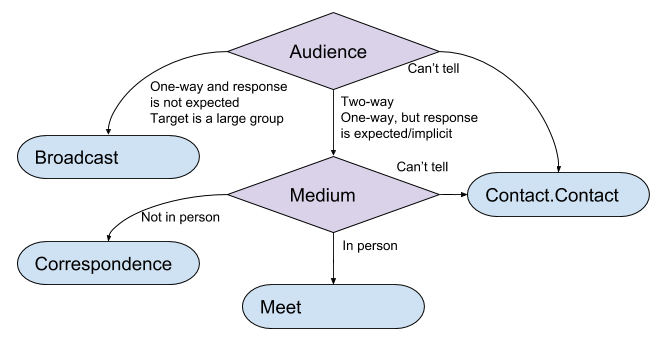
\includegraphics[width=\textwidth]{img/contact_decision_tree.png}
\caption{Contact type decision tree.}
\label{fig:contact_decision_tree}
\end{figure}

\type{Contact} events possess two attributes that are not annotated: Audience and Medium. Determining the value of these attributes will help you categorize \type{Contact} events into the correct subtype by following the decision tree given in figure \ref{fig:contact_decision_tree}.

The \textbf{Audience} attribute is Two-way if there is a back-and-forth in the contact (as with a normal conversation, phone call, interview, etc.). The Audience attribute is One-way if the communication is not or cannot be answered, or if the target (audience) of the message is a large, indefinite group of people. If it impossible to know from context, it is Can't-tell. 

Note that if the nature of the contact implies that a back-and-forth is possible or expected, even though the text only refers to one-way contact, the Audience attribute is also Two-way. This can be difficult to determine. Remember that determining the contact as One-way means the event's subtype becomes \type{Contact.Broadcast}. In some cases (like a Twitter message or a political speech) this is intuitively the right choice. In others there is more room for uncertainty. That is why we use an added criterium: a \type{Broadcast} event requires the audience to be a large group. This is not a hard constraint, but a good rule of thumb. When in doubt, it is best to note the Audience as Can't-tell, in which case the event type becomes the generic \type{Contact.Contact}.

\begin{exe}
    
    \ex \annxpl{De voormalige president maakte tijdens het \anntrg{gesprek} duidelijk dat hij zou meewerken.} 
        \expl A conversation clearly indicates two-way contact. However, we cannot determine if it happened in person or not.
        \type{Contact.Contact}.
        
    \ex \annxpl{The IMF \anntrg{report} gave some hope to countries battered by the depression.} 
        \expl A report indicates One-way contact: no reply is expected. 
        \type{Contact.Broadcast.}
        
    \ex \annxpl{Opmerkelijk is dat Zuckerberg zich liet verassen door een \anntrg{vraag} over zijn persoonlijke gegevens.} 
        \expl The sentence only mentions the one-way contact of a question being asked (there is no indication of a reply). However, it is clear from context that Zuckerberg answered or was expected to answer. The Audience is therefore Two-way. The medium is uncertain. 
        \type{Contact.Contact.}
        
    \ex \annxpl{Jan \anntrg{noemt} Bert een leugenaar.} 
        \expl Only one-way communication is attested. However, \annxpl{Bert} is not a large group of people. It is also not possible to clearly say whether a response is expected here, so we say that Audience is Can't-tell. 
        \type{Contact.Contact}
        
    \ex \annxpl{President Trump once again baffled his followers with an inflammatory \anntrg{tweet.}} 
        \expl A tweet can lead to a back-and-forth conversation through Twitter, but the sentence does not mention this. Because the tweet is sent out to a large group (Trump's twitter followers) and nothing indicates a conversation taking place, the Audience attribute is One-way. 
        \type{Contact.Broadcast.}
    
\end{exe}

The \textbf{Medium} attribute is either In-person, Not-in-person or Can't-tell. A meeting around a table happens in person; a phone call does not. It might be unclear from the sentence which it is. In this case, annotate the event as \type{Contact.Contact}. When In-person and Not-in-person contact happens in the same sentence with different verbs, it is generally advised to annotate two separate events.

\begin{exe}

    \ex \annxpl{De twee hielden nog lang \anntrg{contact} via brief en e-mail.} 
    \expl Their conversation clearly does not happen in person: \type{Contact.Correspondence.}
    
    \ex \annxpl{Naast hun \anntrg{briefwisseling} \anntrg{spraken} ze urenlang over het leven tijdens lange avondwandelingen.} 
    \expl \annxpl{Briefwisseling} denotes a Not-in-person contact event (\type{Contact.Correspondence}), while \annxpl{spraken} occurs In-person (\type{Contact.Meet}).
    
    \ex \annxpl{In \anntrg{brieven} en \anntrg{ontmoetingen} leerden ze elkaar kennen.}
    \expl Ditto: two triggers for two events, even though both events coordinate around the same fact.
    
    \ex \annxpl{Regelmatig \anntrg{contact} bracht hen samen.} 
    \expl In this case it is not possible to know whether the contact happens in person, not in person or both: \type{Contact.Contact.}
    
\end{exe}

More examples:

\begin{exe}
    
    \ex \annxpl{De aanslag van Sayfullo Saipov was een \anntrg{boodschap} voor de wereld.}
    \expl Giving a message is an act of communication. This is a clear instance of one-way communication to a large, undefined group (\annxpl{de wereld}). This leads us to \type{Contact.Broadcast}.
    
    \ex \annxpl{Alle partijen zaten gisteren rond de ronde tafel om de tarieven te \anntrg{bespreken}.} 
    \expl There is necessarily two-way communication going on between the involved parties. Since they are talking in person, this is an instance of \type{Contact.Meet}.
    
    \ex \annxpl{De president \anntrg{contacteerde} de Japanse minister om zich te verontschuldigen.} 
    \expl \annxpl{Contacteerde} implies the communication did not take place face-to-face. We can also reasonably assume that there was some back-and-forth communication: \type{Contact.Correspondence}.
    
    \ex \annxpl{Hammas issued an inflammatory \anntrg{statement}.} 
    \expl Issuing a statement, making a declaration or a speech, etc., all imply one-way communication to a large group: \type{Contact.Broadcast}.
    
    \ex \annxpl{In a groundbreaking \anntrg{report}, the UN made clear its position on climate change.}
    \expl \annxpl{Report}, rather than \annxpl{made clear}, is the trigger of a \type{Contact.Broadcast} event.
    
\end{exe}


\subsection{\type{Contact} argument roles}

\begin{figure}[t]
\centering
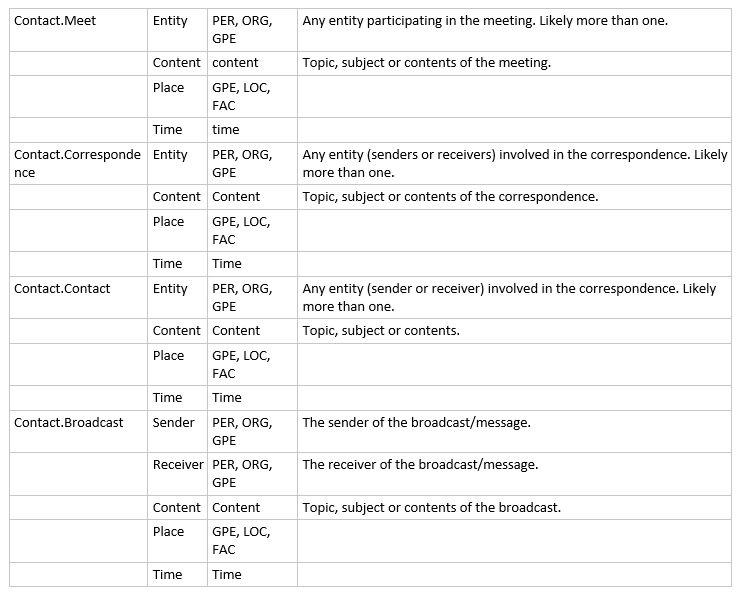
\includegraphics[width=\textwidth]{img/contact_type_args.png}
\caption{Contact type argument roles.}
\label{fig:contact_type_args.png}
\end{figure}

Allowed \type{Contact} type arguments are given in figure \ref{fig:contact_type_args.png}. The Content argument represents the content or topic of the message being transmitted. It will often be an entire relative clause, in which case you should not tag the relative pronoun.

\begin{exe}
    
    \ex \annxpl{De 33-jarige Zuckerberg \anntrg{gaf te kennen} dat \textbf{Facebook tienduizenden apps zou screenen.}} 
        \expl \type{Con\-tact.\-Broad\-cast.} The Content argument is bolded.
    
    \ex \annxpl{Alle partijen zaten gisteren rond de ronde tafel om \textbf{de tarieven} te \anntrg{bespreken.}}
        
    \ex \annxpl{Zuckerberg liet zich verassen door een \anntrg{vraag} over \textbf{zijn persoonlijke gegevens.}}

\end{exe}






\section{Dealing with quotations}

We annotate inside a quotation the same way we annotate outside of it. We do not consider the quotation to be a separate sentence. That means it is possible to identify an event outside a quotation and annotate arguments for that event inside of it, and vice-versa.

\begin{exe}
    \ex \annxpl{\emph{De politie} liet hem weten dat \emph{hij} "snel \anntrg{gearresteerd} zou worden".}
        \expl \type{Justice.ArrestJail}
        \expl Agent = De politie
        \expl Person = hij
        \expl The Person argument lies outside the quote.
\end{exe}

When the quote is the Content argument of a \type{Contact} event, it's important to remember that the inside of the message is separate from the outside of it. We take care not to associate elements inside the message with the same \type{Contact} event.

\begin{exe}
    \ex \annxpl{De \anntrg{boodschap} van de generaal was duidelijk: "IS zal nog harder \anntrg{getroffen} worden."} 
        \expl \annxpl{Boodschap} introduces a \type{Contact.\-Broad\-cast} event to which \annxpl{IS zal nog harder getroffen worden} is the Content argument. However, \annxpl{IS} is not an argument in this event. The message contains a \type{Conflict.Attack} event to which \annxpl{IS} is an argument.
\end{exe}

Sometimes, a quotation is used as the title of an article -- the quotation spans the entire sentence. In this case, no trigger can be identified, and nothing must be annotated.

\begin{exe}
    \ex \annxpl{``Spijtig dat er niet meer doden vielen.''} 
        \expl No trigger can be identified and no event is annotated.
    
    \ex \annxpl{``Spijtig dat er niet meer doden vielen,'' \anntrg{bekende} de dader achteraf.} 
        \expl The trigger is clear. The quote then serves as the Content argument to the \type{Contact.Contact} event.
\end{exe}



